
\begin{frame}
  \frametitle{SPICE: Simulation Program with Integrated Circuit Emphasis}
  \begin{columns}
    \begin{column}{.7\textwidth}
      % In few words
      \begin{itemize}
      \item Developed by Dr. Laurence Nagel in 1973 at Berkeley % University of California
      \item \textbf{First software} to combine \\
        DC, AC and transient analog circuit analysis capabilities
      \item An early \textbf{open source} software initiative (Public Domain)
      \item \textbf{Used in undergraduate courses}
      \item \textbf{Evolved to a worldwide standard} % integrated circuit simulator
      \item \textbf{IEEE Milestone} on February 4, 2011
      \item Berkeley released spice3f5 on 1993 % 6
      \item Superseded by commercial and open source forks
      \end{itemize}
      % What it does ?
      % \begin{itemize}
      % \item Netlist language to describe circuit
      % \item Simulator
      % \end{itemize}
      {\tiny To go further
        \href{https://www2.eecs.berkeley.edu/Pubs/TechRpts/1975/9602.html}%
        {SPICE2: A Computer Program to Simulate Semiconductor Circuits; Nagel, Laurence W.; 1975}
      }
    \end{column}
    \begin{column}{.3\textwidth}
      \begin{center}
        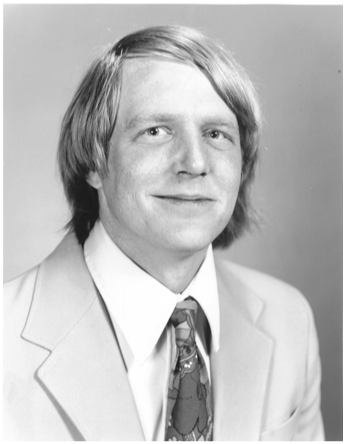
\includegraphics[height=3cm]{images/Larry-Nagel-portrait-young.png} \\[1cm]
        
\includegraphics[width=.7\textwidth]{images/Nagel_Plaque-SCV-2016.png}
      \end{center}
    \end{column}
  \end{columns}
\end{frame}

\begin{frame}[fragile]
  \frametitle{SPICE: Netlist}
  \begin{columns}
    \begin{column}{.5\textwidth}
      \begin{center}
        \includegraphics[width=.9\textwidth]{figures/ac-coupled-amplifier.pdf}
      \end{center}
    \end{column}
    \begin{column}{.5\textwidth}
     {\footnotesize
\begin{verbatim}
AC-coupled amplifier
Vpwr 6 0 DC 15V
Vin 1 0 AC 1V SIN(0V .5V 1KHz)
C1 1 2 10u
R1 6 2 100k
R2 2 0 20k
RC 6 4 10k
Q1 4 2 3 bjt
RE 3 0 2k
C2 4 5 10u
RL 5 0 1Meg
.model bjt npn(bf=80 cjc=5p rb=100)
.ac dec 5 10m 1G
*.tran .02ms 2ms 0 .01ms
.control
run
plot V(1) V(5)
.end
\end{verbatim}%
     }
   \end{column}
 \end{columns}
\end{frame}

\begin{frame}[fragile]
  \frametitle{SPICE: A Worldwide Standard for integrated circuit simulation}
  \centerline{Device manufacturers use SPICE language to provide models as sub-circuit}
  \begin{columns}
    \begin{column}{.5\textwidth}
      \begin{center}
        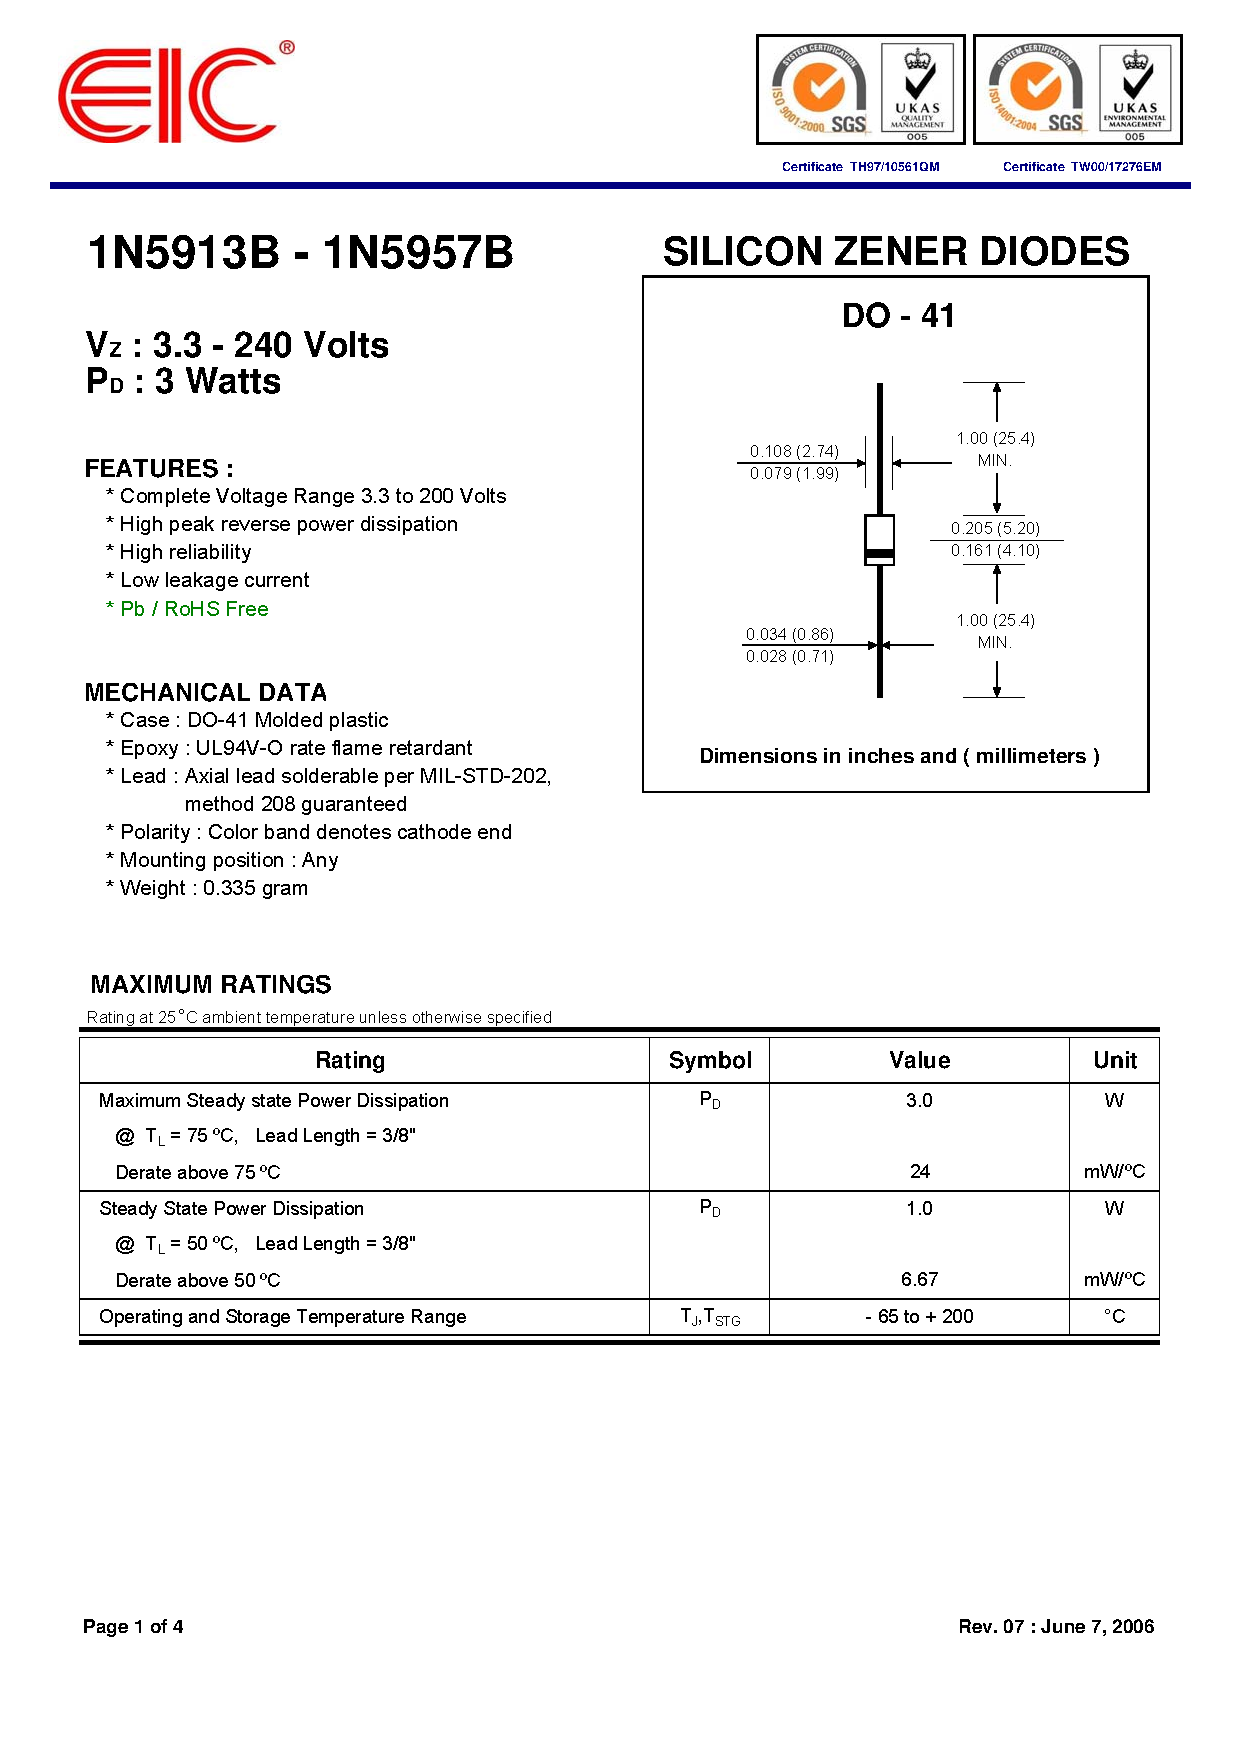
\includegraphics[height=6cm]{figures/1N5919B-1.pdf}
      \end{center}
    \end{column}
    \begin{column}{.5\textwidth}
      {\fontsize{4.25pt}{4.25pt}\selectfont
\begin{verbatim}
* http://www.onsemi.com/pub_link/Collateral/1N5919BRL.SP3
.SUBCKT d1n5919brl 2 1
**************************************
*      Model Generated by MODPEX     *
*Copyright(c) Symmetry Design Systems*
*         All Rights Reserved        *
*    UNPUBLISHED LICENSED SOFTWARE   *
*   Contains Proprietary Information *
*      Which is The Property of      *
*     SYMMETRY OR ITS LICENSORS      *
*    Modeling services provided by   *
* Interface Technologies www.i-t.com *
**************************************
* Model generated on Jun 22, 2004
* MODEL FORMAT: SPICE3
*     anode cathode
*node: 2      1
*    Forward Section
D1 2 1 MD1
.MODEL MD1 D IS=1.33275e-21 N=1 XTI=1 RS=0.1
+ CJO=1e-11 TT=1e-08
*    Leakage Current
R 1 2 600000 MDR
.MODEL MDR R TC1=0 TC2=0
*    Breakdown
RZ 2 3 0.520393
IZG 4 3 0.3204
R4 4 3 100
D3 3 4 MD3
.MODEL MD3 D IS=2.5e-12 N=2.40102 XTI=0 EG=0.1
D2 5 4 MD2
.MODEL MD2 D IS=2.5e-12 N=3.19856 XTI=0 EG=0.1
EV1 1 5 6 0 1
IBV 0 6 0.001
RBV 6 0 5153.19 MDRBV
.MODEL MDRBV R TC1=1.79e-08
*-- SPICE3 DIODE MODEL DEFAULT PARAMETER
*  VALUES ARE ASSUMED
*IS=1E-14 RS=0 N=1 TT=0 CJO=0
*VJ=1 M=0.5 EG=1.11 XTI=3 FC=0.5
*KF=0 AF=1 BV=inf IBV=1e-3 TNOM=27
.ENDS d1n5919brl
\end{verbatim}%
      }
    \end{column}
  \end{columns}
\end{frame}

%%% Local Variables:
%%% mode: latex
%%% TeX-master: "master"
%%% End:
